\chapter{Evaluation} \label{chap:Evaluation}
In this chapter, various case studies are introduced which demonstrate the use of an extension. They have been chosen in order to illustrate the important features of CRI, therefore the contributions of this thesis. We have collected examples written using RxJS and BaconJS libraries from the internet. We have evaluated the extension against several RxJS and BaconJS applications and we present the results in this section. We focus on features provided by our extension and evaluate that feature with the applications. In the last section, we summarize and conclude the evaluation.

\section{Operators}
Operators play an important role in both libraries. Developers can use operators to transform, filter and for many other operations. To demonstrate how CRI helps developers to understand reactive applications, we have taken RxJS operators example code. This section also illustrates the evolution of dependency graph for the given example.

\subsection{RxJS - Operators}
In our example, we have selected \textit{map}, \textit{filter} and \textit{last} operators from RxJS library. One can find use case of other operators in RxJS official documentation\footnote{\url{http://reactivex.io/documentation/operators.html}}. Dependency graph generated by CRI after executing the program is shown in figure \ref{fig:rxjs-operators-dg}. In the following example~\ref{lst:rxjs-operators}, \textit{source} is an observable with values {1,2,3,4,5}. In line 3, \textit{map} operator is applied, which maps each values from an observable and adds 10 to each value and new \textbf{MapObservable} is created. At line 5, \textit{filter} operator filters the even values out of \textbf{MapObservable}. The \textit{last} operator at line 7 receives values 12 and 14 after applying filter operator and emits value 14 which the last value in observable. At line 9, subscriber \textit{subscribe} is subscribing to \textit{example} observable. Thus, \textit{subscribe} will receive value 14 and is printed to console in line 10.

\begin{lstlisting}[language=JavaScript, caption=RxJS - Operators example, label={lst:rxjs-operators}]
var source = Rx.Observable.from([1, 2, 3, 4, 5]);
// apply map, filter and last operator
var example = source.map(function (val) {
	return val + 10;
}).filter(function (num) {
	return num % 2 === 0;
}).last();
//output: "Last to pass test: 14"
var subscribe = example.subscribe(function (val) {
	return console.log("Last value: " + val);
});
\end{lstlisting}

\begin{figure}[!h]
	\centering
	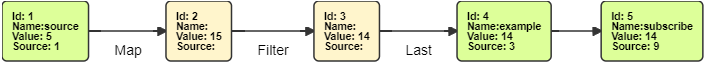
\includegraphics[scale=0.7,trim=0 0 0 0]{images/RxJS-operators/final.png}
	\caption{Dependency graph - RxJS Operators example}
	\label{fig:rxjs-operators-dg}
\end{figure}

As we said earlier, CRI helps the developer to understand the flow of reactive applications. For listing~\ref{lst:rxjs-operators}, evolution of dependency graph can be depicted as shown in figure \ref{fig:rxjs-operators-dg-evolution}. Developer can use the provided slider to navigate to and forth to visualize evolution of graph. In the first 3 steps, node \textit{source} is created and how the program runs internally after applying map and filter operator is depicted. In the last step, subscriber \textit{subscribe} is created which is subscribed to node \textit{example}. Thus, connection between \textit{example} and \textit{subscribe} exists.

\begin{figure}[!h]
	\centering
	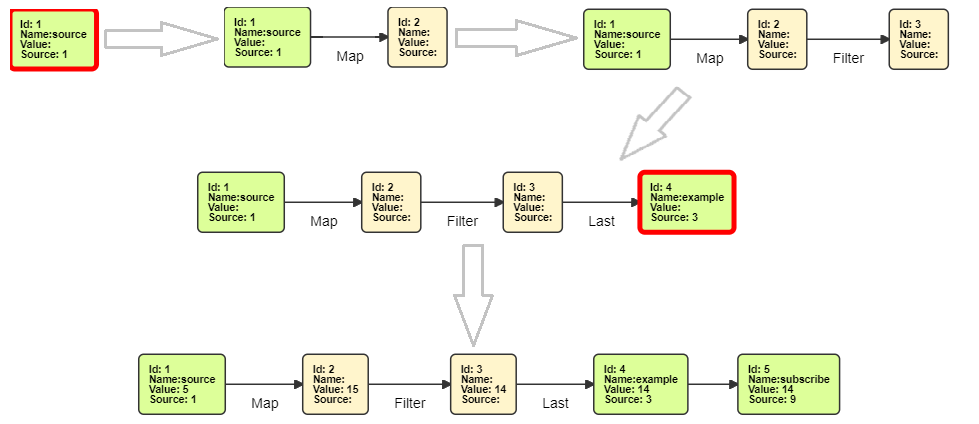
\includegraphics[scale=0.7,trim=0 0 0 0]{images/RxJS-operators/steps-all.png}
	\caption{Dependency graph evolution - RxJS Operators example}
	\label{fig:rxjs-operators-dg-evolution}
\end{figure}

\section{RxJS - Subjects}
Listing \ref{lst:rxjs-data-binding} shows relevant javascript code for this example. In current example, user enters data in two HTML input fields: firstname and lastname. Output of the application is the combination of both names. The UI of an application looks as shown in figure~\ref{fig:sd-ui} and dependency graph is shown in figure~\ref{fig:sd-dg}. 

\begin{lstlisting}[language=JavaScript, caption=RxJS - Databinding example, label={lst:rxjs-data-binding}]
// Create simple bindings for first and last name
var firstName1 = new Rx.BehaviorSubject('');
var lastName1 = new Rx.BehaviorSubject('');

// Create first and last name composite
var fullName1 = firstName1.combineLatest(lastName1, function (first, last) {
	return first + ' ' + last;
});

// Subscribe to them all
var fn1 = document.querySelector('#firstName1');
firstName1.subscribe(function (text) { fn1.value = text });

var ln1 = document.querySelector('#lastName1');
lastName1.subscribe(function (text) { ln1.value = text });

var full1 = document.querySelector('#fullName1');
fullName1.subscribe(function (text) { full1.value = text });

// Create two way bindings for both first name and last name
Rx.Observable.fromEvent(fn1, 'keyup')
.subscribe(function (e) { firstName1.next(e.target.value); })

Rx.Observable.fromEvent(ln1, 'keyup')
.subscribe(function (e) { lastName1.next(e.target.value); })
\end{lstlisting}


\begin{figure}[!h]
	\centering
	\subfloat[UI]{\includegraphics[width=0.4\textwidth]{images/simple-data-binding/simple-db-UI.png}\label{fig:sd-ui}}
	\hfill
	\subfloat[Dependency graph]{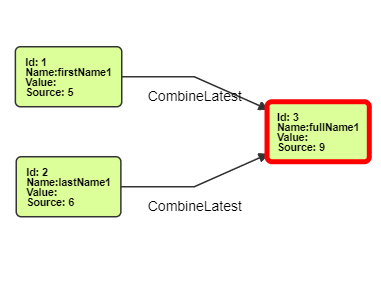
\includegraphics[width=0.4\textwidth]{images/simple-data-binding/sd-dg.png}\label{fig:sd-dg}}
	\caption{Simple Data-binding example - RxJS}
\end{figure}

\section{RxJS - Animation Test}
This is a simple animation example in which the user moves the mouse in the given area and the mouse trail with colorful boxes is animated. Relevant code for the example is listed in the listing \ref{lst:rxjs-animation-test}. This kind of example is hard to implement with vanilla javascript. Thankfully RxJS does all the work for user and emits mouse pointer values in the form of data streams. UI for the example is depicted in figure \ref{fig:rxjs-at-ui} and dependency graph generated is shown in figure \ref{fig:rxjs-at-dg}.

\begin{lstlisting}[language=JavaScript, caption=RxJS - Animation Test example, label={lst:rxjs-animation-test}]	
$(function () {
	Rx.Observable.prototype.movingWindow = function(size, selector, onShift) {
		var source1 = this;
		return Rx.Observable.create(function (o) {
			var arr = [];
			return source1.subscribe(
			function (x) {
				var item = selector(x);
				arr.push(item);
				if (arr.length > size) {
					var i = arr.shift();
					onShift(i);
				}
			},
			function (e) { o.onError(e); }
			);
		})
	}
	// Drawing area
	var canvas = $('#drawing');
	var source = Rx.Observable.fromEvent(canvas, 'mousemove')
	.movingWindow(
	25,
	function (x) {
		var b = new Box([x.clientX, x.clientY], canvas);
		b.showBox();
		return b;
	},
	function (b) {
		b.hideBox();
	}
	);	
	var sourceSubscriber = source.subscribe();	
});
\end{lstlisting}

\begin{figure}[!h]
	\centering
	\includegraphics[scale=0.4,trim=0 0 0 0]{images/animation-test/at-ui.png}
	\caption{UI - Animation Test}
	\label{fig:rxjs-at-ui}
\end{figure}
\begin{figure}[!h]
	\centering
	\includegraphics[scale=0.4,trim=0 0 0 0]{images/animation-test/at-dg.png}
	\caption{Dependency graph - Animation Test}
	\label{fig:rxjs-at-dg}
\end{figure}

\section{RxJS - Drawing example}
This is one of the advanced example from the previous examples. Figure \ref{fig:rxjs-draw-ui} shows the options available for the user. Here, the user has seven different options to draw an image. User can set outer-radius, inner-radius, different color fillings to an image. As soon as user modifies the value from the available options, the same is reflected in the image. The relevant dependency graph is shown in figure \ref{fig:rxjs-draw-dg}.

\begin{figure}[!h]
	\centering
	\includegraphics[scale=0.5,trim=0 0 0 0]{images/draw/draw-ui.png}
	\caption{UI - Drawing example}
	\label{fig:rxjs-draw-ui}
\end{figure}

\begin{lstlisting}[language=JavaScript, caption=RxJS - Drawing example, label={lst:rxjs-draw}]
var Observable = Rx.Observable;
var fromEvent = Observable.fromEvent;

var points$ = fromEvent(points, 'input', function (e) {
	return e.target.value;
}).startWith(points.value);

var outerRadius$ = fromEvent(outerRadius, 'input', function (e) {
	return e.target.value;
}).startWith(outerRadius.value).distinctUntilChanged();

var innerRadius$ = fromEvent(innerRadius, 'input', function (e) {
	return e.target.value;
}).startWith(innerRadius.value);

var angle$ = fromEvent(angle, 'input', function (e) {
	return e.target.value;
}).startWith(angle.value);

var lineWidth$ = fromEvent(lineWidth, 'input', function (e) {
	return e.target.value;
}).startWith(lineWidth.value);

var strokeColor$ = fromEvent(strokeColor, 'input', function (e) {
	return e.target.value;
}).startWith(strokeColor.value);

var fillColor$ = fromEvent(fillColor, 'input', function (e) {
	return e.target.value;
}).startWith(fillColor.value);

Rx.Observable.combineLatest(points$, outerRadius$, innerRadius$, angle$, strokeColor$, fillColor$, lineWidth$).subscribe(function (values) {
	draw.apply(null, values);
});

\end{lstlisting}

Listing \ref{lst:rxjs-draw} shows relevant RxJS code for the example. It looks complicated at the first glance. But with the help of dependency graph, user can understand which part of the code depends on other part of the code. 

\begin{figure}[!h]
	\centering
	\includegraphics[width=\textwidth,height=\textheight,keepaspectratio]{images/draw/draw-dg.png}
	\caption{Dependency graph - Drawing example}
	\label{fig:rxjs-draw-dg}
\end{figure}

We will evaluate breakpoint feature of CRI extension against this example. In large applications, it is important for the user to know at what point of the program bug exists. Breakpoint feature helps user to find out by specifying conditions. In our example, we will set up a breakpoint when node with ID 19 is created. We select \textit{nodeCreated[nodeId]} from the dropdown available, which is discussed in~\ref{section:cri-ui} and set value to \textit{nodeCreated[19]}. After setting up breakpoint, the user can see all the breakpoints as shown in figure \ref{fig:rxjs-draw-bp}. Figure \ref{fig:rxjs-draw-bp} and \ref{fig:rxjs-draw-bp2} shows that when a program hits the breakpoint, it halts the execution and goes into debugger mode. 

\begin{figure}[h]
	\centering
	\includegraphics[width=\textwidth,height=\textheight,keepaspectratio]{images/draw/breakpoint-example-1.png}
	\caption{Setup Breakpoint - Drawing example}
	\label{fig:rxjs-draw-bp}
\end{figure}

\begin{figure}[h]
	\centering
	\includegraphics[width=\textwidth,height=\textheight,keepaspectratio]{images/draw/breakpoint-example-2.png}
	\caption{After Breakpoint is hit}
	\label{fig:rxjs-draw-bp2}
\end{figure}


\section{RxJS - Stopwatch example}
Let us have a look at another typical example from RxJS applications. This application acts as a stopwatch with initial time of 90 seconds. When a user clicks on the timer, counter starts. When user clicks on running timer, it is paused. Listing \ref{lst:rxjs-stopwatch} shows relevant RxJS code for the application. And figure \ref{fig:rxjs-sw-dg} shows dependency graph generated for the application. In this example, there are 17 operators in total. Among them, 9 unique operators used. 

%\begin{sidewaysfigure}[!ht]
%	\centering
%	\includegraphics[width=\textwidth]{images/stopwatch/stopwatch-dg.png}
%	\caption{Dependency graph - Stopwatch}
%	\label{fig:rxjs-sw-dg}
%\end{sidewaysfigure}
\begin{figure}[!h]
	\centering
	\includegraphics[width=\textwidth,height=\textheight,keepaspectratio]{images/draw/draw-dg.png}
	\caption{Dependency graph - Drawing example}
	\label{fig:rxjs-sw-dg}
\end{figure}

\begin{lstlisting}[language=JavaScript, caption=RxJS - Stopwatch example, label={lst:rxjs-stopwatch}]
// DOM elements

var interval$ = Rx.Observable.interval(1000);
var click$ = Rx.Observable.fromEvent(document, 'click');
var dblclick$ = Rx.Observable.fromEvent(document, 'dblclick');
var toggleOrReset$ = Rx.Observable.merge(click$.mapTo(function (isRunning) {
	return !isRunning;
}), dblclick$.mapTo(function () {
	return false;
})).startWith(false).scan(function (isRunning, toggleOrFalse) {
	return toggleOrFalse(isRunning);
}).do(function (isRunning) {
	return console.log('Running:', isRunning);
}).share();
var start$ = toggleOrReset$.filter(function (isRunning) {
	return isRunning;
});
var stop$ = toggleOrReset$.filter(function (isRunning) {
	return !isRunning;
});
var incOrDecOrReset$ = Rx.Observable.merge(interval$.takeUntil(Rx.Observable.merge(stop$, dblclick$)).mapTo(incOrDec), dblclick$.mapTo(reset));
start$.switchMapTo(incOrDecOrReset$).startWith(initialValue).scan(function (seconds, incOrDecOrReset) {
	return incOrDecOrReset(seconds);
}).takeWhile(stillCan).map(toTime).subscribe(render);

\end{lstlisting}


We will evaluate CRI features such as search, find dependents and dependencies of a given node against this application. Similarly, user can use these features for all the RxJS applications. 
For example, we will search node named \textit{toggleOrReset\$} in the dependency graph. Figure \ref{fig:stopwatch-search} depicts the result of the search. This features makes navigation in large dependency graphs much comfortable.

\begin{figure}[!h]
	\centering
	\includegraphics[width=\textwidth,height=\textheight,keepaspectratio]{images/stopwatch/search.png}
	\caption{Search feature}
	\label{fig:stopwatch-search}
\end{figure}

Dependency highlighting feature helps the user to find all the dependents and dependencies of a given node much easier. Figure \ref{fig:dependents} shows all the dependent nodes and figure \ref{fig:dependencies} highlights all the dependency nodes of given node \textit{toggleOrReset\$}.  

\begin{figure}[!h]
	\centering
	\includegraphics[width=\textwidth,height=\textheight,keepaspectratio]{images/stopwatch/dependents.png}
	\caption{Highlighting Dependent nodes}
	\label{fig:dependents}
\end{figure}

\begin{figure}[!h]
	\centering
	\includegraphics[width=\textwidth,height=\textheight,keepaspectratio]{images/stopwatch/dependencies.png}
	\caption{Highlighting dependencies of a node}
	\label{fig:dependencies}
\end{figure}

\section{BaconJS - Drag-n-Drop}
Let us look into another interesting application called ``Drag-n-Drop''. When uploading files to server via browser, some websites provide an option to drag and drop the files. Our application imitates such feature but not with files. In this application, the user can drag contents from one box and drop in another box. For example, in the figure \ref{fig:drag-drop-ui}, last box contains both \textbf{A} and \textbf{B} values. User can drop \textbf{B} in box B but not in A. Similarly, \textbf{A} can be dropped in box A only. Listing \ref{lst:drag-drop-code}, shows relevant code for the example. Figure \ref{fig:drag-drop-dg}, depicts final view of the dependency graph.

\begin{figure}[!h]
	\centering
	\includegraphics[width=\textwidth,height=\textheight,keepaspectratio]{images/drag-drop/drag-drop-ui.png}
	\caption{BaconJS - Drag-n-Drop UI}
	\label{fig:drag-drop-ui}
\end{figure}

\begin{figure}[!h]
	\centering
	\includegraphics[width=\textwidth,height=\textheight,keepaspectratio]{images/drag-drop/drag-drop-dg.png}
	\caption{BaconJS - Drag-n-Drop Dependency graph}
	\label{fig:drag-drop-dg}
\end{figure}


\begin{lstlisting}[language=JavaScript, caption=BaconJS - Drag-n-Drop Example, label={lst:drag-drop-code}]
var homeBin, drag, drop, this$ = this;
$.event.props.push('dataTransfer');
homeBin = $('#home-bin');
drag = $(document).asEventStream('dragstart', '.item').doAction(function (e) {
	e.dataTransfer.effectAllowed = 'move';
	return e.dataTransfer.setData('tmp', '');
	}).toProperty();
drop = $('.drag-bin').asEventStream('dragover drop').doAction(function (it) {
	return it.preventDefault();
	}).filter(function (it) {
		return it.type === 'drop';
}).toProperty();
drag.combine(drop, function (a, b) {
return [a, b];
}).filter(function (arg$) {
var a, b;
a = arg$[0], b = arg$[1];
return a.timeStamp < b.timeStamp;
}).map(function (arg$) {
var a, b;
a = arg$[0], b = arg$[1];
return {
item: a.target,
dest: b.target
};
}).filter(function (arg$) {
var item, dest;
item = arg$.item, dest = arg$.dest;
return item.dataset.type === dest.dataset.type || dest.dataset.type == null;
}).assign(function (arg$) {
var item, dest;
item = arg$.item, dest = arg$.dest;
dest.appendChild(
item);
});
$('.item .remove').asEventStream('click').assign(function (e) {
homeBin.append(
$(e.target).closest('.item'));
});
\end{lstlisting}

We will now evaluate \textit{History Queries} feature against this example. Use case of History queries is described in the section \ref{section:cri-ui}.
After dragging \textbf{B} to box B, we ran the query \textit{nodeUpdated[drop]}. We found 2 stages where node \textit{drop} is updated. Changes after the query can be seen as shown in figure \ref{fig:drag-drop-hq}. Node \textit{drop} is updated at the step 14 and 81.  

\begin{figure}[!h]
	\centering
	\includegraphics[scale=0.7,trim=0 0 0 0]{images/drag-drop/drag-drop-hq.png}
	\caption{History Queries example}
	\label{fig:drag-drop-hq}
\end{figure}

\section{RxJS - Wikipedia updates}
Listing \ref{lst:rxjs-wiki-updates} shows a short example from RxJS applications that creates websocket connection to third party server. Server sends different type of notifications which are then received by websocket connection. The data received is then converted to data stream named \textit{updateStream}. The target application filters the \textit{updateStream} into three streams named \textit{newUserStream}, \textit{editStream} and \textit{updateCount}. Finally, values from each stream are used to draw a graph and updates other information to target web page. Dependency graph of target application is shown in the figure \ref{fig:rxjs-wiki-updates-dg} and UI is shown in figure \ref{fig:rxjs-wiki-updates-ui}. Splitting of one stream into three streams is easily understood with the help of dependency graph. Thus, helping user to quickly understand how the application is working. 

\begin{lstlisting}[language=JavaScript, caption=RxJS - Live updates from Wikipedia, label={lst:rxjs-wiki-updates}]
// Create our websocket to get wiki updates
var ws = new window.WebSocket("ws://wiki-update-sockets.herokuapp.com/");

var messageStream = fromEvent(ws, 'message');

var updateStream = messageStream.map(function(event) {
var dataString = event.data;
return JSON.parse(dataString);
});

// Filter the update stream for newuser events
var newUserStream = updateStream.filter(function(update) {
return update.type === "newuser";
});
newUserStream.subscribe(function() {
var format = d3.time.format("%X");
updateNewUser(["New user at: " + format(new Date())]);
});

// Filter the update stream for unspecified events, which we're taking to mean
// edits in this case
var editStream = updateStream.filter(function(update) {
return update.type === "unspecified";
});
editStream.subscribe(function(results) {
updateEditText(["Last edit: " + results.content]);
});

// Calculate the rate of updates over time
var updateCount = updateStream.scan(function(value) {
return ++value;
}, 0);

var sampledUpdates = updateCount.sample(Rx.Observable.interval(samplingTime));
var totalUpdatesBeforeLastSample = 0;
sampledUpdates.subscribe(function(value) {
updatesOverTime.push({
x: new Date(),
y:(value - totalUpdatesBeforeLastSample) /
(samplingTime / 1000)
});
if (updatesOverTime.length > maxNumberOfDataPoints)  {
updatesOverTime.shift();
}
totalUpdatesBeforeLastSample = value;
update(updatesOverTime);
});
\end{lstlisting}

\begin{figure}[!h]
	\centering
	\includegraphics[width=\textwidth,height=\textheight,keepaspectratio]{images/wiki-updates/wiki-updates-ui.png}
	\caption{UI - Wikipedia updates}
	\label{fig:rxjs-wiki-updates-ui}
\end{figure}
\begin{figure}[!h]
	\centering
	\includegraphics[width=\textwidth,height=\textheight,keepaspectratio]{images/wiki-updates/wiki-updates-dg.png}
	\caption{Dependency graph - Wikipedia updates}
	\label{fig:rxjs-wiki-updates-dg}
\end{figure}

\section{Existing design vs Current design}
In this section we will discuss the improvisations made in this thesis from previous version of CRI. Listing \ref{lst:rxjs-count}, shows an example which counts the length of text input from the UI~\ref{fig:rxjs-count-ui}. In line 10, we are subscribing to \textit{source} observable. Thus, every values emitted by \textit{source} is received by the subscriber and set using function \textit{setHtml} at line 5. 


\begin{lstlisting}[language=JavaScript, caption=RxJS - Letter Count, label={lst:rxjs-count}]
var source = Rx.Observable.fromEvent($toCount, 'keyup')
.map(function (e) { return 'length: ' + e.target.value.length; })
.distinctUntilChanged();

function setHtml(text) {
	console.log(text);
	this.innerHTML = text;
}

source.subscribe(setHtml.bind($result));
\end{lstlisting}

\begin{figure}[!h]
	\centering
	\includegraphics[scale=0.7,trim=0 0 0 0]{images/improvisations/initial-ui.png}
	\caption{RxJS - Letter Count example}
	\label{fig:rxjs-count-ui}
\end{figure}


In previous version of CRI developed, the author is subscribing to each observable again to catch all the events using the code listed in listing \ref{lst:prev-cri-code}. Here, \textit{obs} represents an observable from the target application. Each value emitted is then logged to dependency graph using the method \textit{sendToDevTools} at line 2. In current version, we have improved it and overridden RxJS library functions to catch all the events. Listing \ref{lst:curr-cri-code}, shows relevant code. \textit{Rx.Subscriber.prototype.next} method catches all the values emitted by all the observables from the target application. Thus, providing more control over all the emitted values and make necessary modifications. 

\begin{lstlisting}[language=JavaScript, caption=Previous implementation, label={lst:prev-cri-code}]
obs.subscribe(function (x) {
	sendObjectToDevTools({
		content: {
			'nodeId': obs.id,
			'nodeType': obsType,
			'nodeMethod': '',
			'nodeRef': '',
			'nodeValue': x,
			'sourceCodeLine': ''
		}, action: "saveNode", destination: "panel"
	});
}
\end{lstlisting}
\begin{lstlisting}[language=JavaScript, caption=Current implementation, label={lst:curr-cri-code}]
 Rx.Subscriber.prototype.next = function (value) {
 	var self = this;
 	sendObjectToDevTools({
	 	content: {
	 	'nodeId': self._id,
	 	'nodeType': self.obsType,
	 	'nodeMethod': '',
	 	'nodeRef': '',
	 	'nodeValue': value,
	 	'sourceCodeLine': ''
	 	}, action: "saveNode", destination: "panel"
 	});
 }
\end{lstlisting}

The disadvantage of previous implementation is, it logs the same values repeatedly because each observable is subscribed twice: once in target application and once in the CRI extension. This works fine for smaller application but there is huge communication overhead and excessive resource consumption. After typing the letters \textit{TU} in the text-box from figure \ref{fig:rxjs-count-ui}, total number of message communication in previous version of CRI is 36 and current version is 16. Resultant dependency graph for each version of CRI is shown in figures \ref{fig:prev-cri} and \ref{fig:curr-cri}.
There are 20 extra message communications, which consumes resources to communicate. The numbers vary to large extent in bigger applications. And current version of CRI provide more detailed information regarding what is going on in the target application. For example, look at the node with id 1, in both the figures \ref{fig:prev-cri} and \ref{fig:curr-cri}. As the user types, CRI catches the events and maps them to display meaningful data to help the developers. 

\begin{figure}[!h]
	\centering
	\includegraphics[width=\textwidth,height=\textheight,keepaspectratio]{images/improvisations/previous.png}
	\caption{CRI - Previous version}
	\label{fig:prev-cri}
\end{figure}
\begin{figure}[!h]
	\centering
	\includegraphics[width=\textwidth,height=\textheight,keepaspectratio]{images/improvisations/new.png}
	\caption{CRI - Current version}
	\label{fig:curr-cri}
\end{figure}

\section{Profiling Time - Library calls from the User space}
In this section we evaluate time taken by overridden RxJS library function calls for the applications discussed in this chapter earlier. Google Chrome provides developers the performance API - Google Chrome DevTools \textbf{Javascript Profiler}\cite{jsprofiler}. We used this profiling feature to evaluate performance of CRI extension. Javascript profiler provides more detailed information on which javascript functions were called and how long each took. This feature from Chrome can be accessed by navigating to DevTools and select the panel ``Javascript Profiler''. Then, user can click on start button to start the recording and upon stopping, the user can see the snapshot of the functions that were called and the time each function took. The figures \ref{fig:prof-without-cri} and \ref{fig:prof-with-cri} shows the time taken by functions without CRI and with CRI used respectively. Our primary focus is on \textbf{Self-time} view. Self-time is the time on specific function and the \textbf{Total-time} is the time executing sub function calls. In CRI, we are calling original library calls in our overridden functions, \textbf{Total-time} would include the time spent in the library activities. We can see that, time spent in the functions that we have overridden is minimal in comparison.

\begin{figure}[!h]
	\centering
	\includegraphics[width=\textwidth,height=\textheight,keepaspectratio]{images/profiling/without-cri.png}
	\caption{Javascript profiling - without CRI}
	\label{fig:prof-without-cri}
\end{figure}
\begin{figure}[!h]
	\centering
	\includegraphics[width=\textwidth,height=\textheight,keepaspectratio]{images/profiling/with-cri.png}
	\caption{Javascript profiling - with CRI}
	\label{fig:prof-with-cri}
\end{figure}

\section{Summary of Evaluation}
The preceding evaluation illustrated with the help of various examples what the contributions of this thesis are. We have evaluated few other RxJS and BaconJS applications from the web and found that our extension works fine and support most of the operators from RxJS library. Additionally, we showed how visualization can help in getting good overview of reactive system and understand its internals at a glance. One main drawback of our extension is that it supports applications with javascript version upto ECMAScript 5.1\cite{es5} due to limitations of Jalangi framework\cite{jalangiissue}. Sometimes target applications have event streams which are continuously emitting values after every short interval of time, can cause heavy message passing and memory consuming. We are confident that the approach used in CRI extension works properly and helps developers to understand and debug reactive applications. 
